\documentclass[10pt,twocolumn,letterpaper]{article}

\usepackage{iccv}
\usepackage{times}
\usepackage{epsfig}
\usepackage{graphicx}
\usepackage{amsmath}
\usepackage{amssymb}
\usepackage{mathtools}
\usepackage{bm}
\usepackage{caption}
\usepackage{subcaption}
\usepackage{multirow}

% Include other packages here, before hyperref.
\def\ellv{\bm{\ell}}
\def\phiv{{\bm{\phi}}}
\def\thetav{\bm{\theta}}
\def\omegav{\bm{\omega}}

\def\av{\mathbf{a}}
\def\bv{\mathbf{b}}
\def\cv{\mathbf{c}}
\def\dv{\mathbf{d}}
\def\ev{\mathbf{e}}
\def\fv{\mathbf{f}}
\def\gv{\mathbf{g}}
\def\hv{\mathbf{h}}
\def\iv{\mathbf{i}}
\def\jv{\mathbf{j}}
\def\kv{\mathbf{k}}
\def\lv{\mathbf{l}}
\def\mv{\mathbf{m}}
\def\nv{\mathbf{n}}
\def\ov{\mathbf{o}}
\def\pv{\mathbf{p}}
\def\qv{\mathbf{q}}
\def\rv{\mathbf{r}}
\def\sv{\mathbf{s}}
\def\tv{\mathbf{t}}
\def\uv{\mathbf{u}}
\def\vv{\mathbf{v}}
\def\wv{\mathbf{w}}
\def\xv{\mathbf{x}}
\def\yv{\mathbf{y}}
\def\zv{\mathbf{z}}

\def\Am{\mathbf{A}}
\def\Bm{\mathbf{B}}
\def\Cm{\mathbf{C}}
\def\Dm{\mathbf{D}}
\def\Em{\mathbf{E}}
\def\Fm{\mathbf{F}}
\def\Gm{\mathbf{G}}
\def\Hm{\mathbf{H}}
\def\Im{\mathbf{I}}
\def\Jm{\mathbf{J}}
\def\Km{\mathbf{K}}
\def\Lm{\mathbf{L}}
\def\Mm{\mathbf{M}}
\def\Nm{\mathbf{N}}
\def\Om{\mathbf{O}}
\def\Pm{\mathbf{P}}
\def\Qm{\mathbf{Q}}
\def\Rm{\mathbf{R}}
\def\Sm{\mathbf{S}}
\def\Tm{\mathbf{T}}
\def\Um{\mathbf{U}}
\def\Vm{\mathbf{V}}
\def\Wm{\mathbf{W}}
\def\Xm{\mathbf{X}}
\def\Ym{\mathbf{Y}}
\def\Zm{\mathbf{Z}}

\newcommand{\homogeneous}[1]{\hat{#1}} % Vector homogenous notation
\newcommand{\hnorm}[1]{\check{#1}} % Perspective division notation

\def\Projection{\mathcal{P}}
\def\IntrinsicMatFunc{\mathcal{K}}
\def\ExtrinsicFunc{\mathcal{R}}
\def\pdiv{\hat{\mathbf{\nu}}}
\def\Distortion{\mathcal{D}}

\def\Real{\varmathbb{R}}
\def\Projective{\varmathbb{P}}

\DeclareMathOperator*{\argmin}{arg\,min}
\DeclareMathOperator{\Err}{Err}
\DeclareMathOperator{\Proj}{Proj}
\DeclareMathOperator{\Norm}{Norm}

\DeclarePairedDelimiter{\norm}{\lVert}{\rVert}

% Add a period to the end of an abbreviation unless there's one
% already, then \xspace.
\makeatletter
\DeclareRobustCommand\onedot{\futurelet\@let@token\@onedot}
\def\@onedot{\ifx\@let@token.\else.\null\fi\xspace}

\def\eg{\emph{e.g}\onedot} \def\Eg{\emph{E.g}\onedot}
\def\ie{\emph{i.e}\onedot} \def\Ie{\emph{I.e}\onedot}
\def\cf{\emph{c.f}\onedot} \def\Cf{\emph{C.f}\onedot}
\def\etc{\emph{etc}\onedot} \def\vs{\emph{vs}\onedot}
\def\wrt{w.r.t\onedot} \def\dof{d.o.f\onedot}
\def\etal{\emph{et al}\onedot}
\makeatother

%Author notes
\def\authornote#1#2{{\textred{\textsl{\small#1:[*#2*]}}}} \newcommand*{\Scale}[2][4]{\scalebox{#1}{$#2$}}%
\newcommand{\dhnote}[1]{\authornote{DH}{#1}} % Daniel
\newcommand{\jknote}[1]{\authornote{JK}{#1}} % Juho
\newcommand{\jhnote}[1]{\authornote{JH}{#1}} % Janne

\graphicspath{{images/}}

% If you comment hyperref and then uncomment it, you should delete
% egpaper.aux before re-running latex.  (Or just hit 'q' on the first latex
% run, let it finish, and you should be clear).
\usepackage[pagebackref=true,breaklinks=true,letterpaper=true,colorlinks,bookmarks=false]{hyperref}

% \iccvfinalcopy % *** Uncomment this line for the final submission

\def\iccvPaperID{408} % *** Enter the ICCV Paper ID here
\def\httilde{\mbox{\tt\raisebox{-.5ex}{\symbol{126}}}}

% Pages are numbered in submission mode, and unnumbered in camera-ready
\ificcvfinal\pagestyle{empty}\fi
\begin{document}

%%%%%%%%% TITLE
\title{Forget the checkerboard: practical self-calibration using a planar scene\\Supplementary material}

\author{First Author\\
Institution1\\
Institution1 address\\
{\tt\small firstauthor@i1.org}
% For a paper whose authors are all at the same institution,
% omit the following lines up until the closing ``}''.
% Additional authors and addresses can be added with ``\and'',
% just like the second author.
% To save space, use either the email address or home page, not both
\and
Second Author\\
Institution2\\
First line of institution2 address\\
{\tt\small secondauthor@i2.org}
}

\maketitle
%\thispagestyle{empty}


%%%%%%%%% ABSTRACT
%%%%%%%%% BODY TEXT	
\section{Additional results}
We present additional calibration results with real cameras in Table \ref{fig:results2}. Camera B is a low-quality Logitech webcam V-UAR33. Camera C is a very old Creative Labs webcam PD-1000. Camera C has significant distortion (see Fig.~\ref{fig:sample}) and severe rolling shutter effects. The rolling shutter problems did not allow video calibration, but the algorithm successfully calibrated the distortion. The two validation image sets consisted of 15 checkerboard images and in both cases the checkerboard corners covered the whole image area in various configurations. Both cameras are calibrated successfully and very accurately, as seen by the low validation reprojection errors. Thus confirming the results presented in the paper. 

\begin{table}
\caption{Additional calibration results with real cameras. Our method consistently matches the performance of Bouguet's calibration toolbox.}
\label{fig:results2}
\centering
\begin{tabular}{|c|c|c|c|c|}
\hline
 & & Bouguet & \multicolumn{2}{|c|}{Our method (\%)} \\
& & & user match & automatic match  \\
 \hline
\multirow{6}{*}{B} & $f_x$ & 552.68 & -0.15 & -2.76 \\
& $f_x$ & 548.39 & -0.19 &  -3.06\\
& $u_0$ & 321.97 & 0.02 &  2.65 \\
& $v_0$ & 235.25 & 0.11 &  2.84 \\
& $d_0$ & -0.184 & -6.23  &  6.28 \\
& $d_1$ & 0.254 & -8.54 &  -24.13 \\
  \hline
& $e_{\text{train}}$ & 0.17px & 0.16px & 0.66px\\ 
& $e_{\text{val}}$ & 0.26px & 0.26px & 0.38px \\ 
  \hline
  \hline
\multirow{6}{*}{C} & $f_x$ & 763.90 & -0.08 &  \\
& $f_x$ & 759.56 & 0.13 &   \\
& $u_0$ & 306.74 & 2.41 &  no video \\
& $v_0$ & 247.25 & 7.17 &  available \\
& $d_0$ & -0.409 & -5.26  &  \\
& $d_1$ & 0.287 & -25.99 &   \\
  \hline
& $e_{\text{train}}$ & 0.47px & 0.46px & n/a\\ 
& $e_{\text{val}}$ & 0.50px & 0.50px & n/a \\ 
\hline
\end{tabular}
\vspace*{-0.5cm}
\end{table}

\section{Limitations of the feature extractor}

Although the feature matching stage is outside of the scope of our paper, we briefly address the limitation of the off-the-shelf feature extractor used and how this limits calibration accuracy. We used the ORB feature extractor implemented in OpenCV. The feature matching stage limits the calibration accuracy for two reasons. First, the localization accuracy of the feature extractor is naturally lower than that of carefully selected checkerboard corners. But more importantly, the current implementation leaves the borders of the image unconstrained.

Figure \ref{fig:sample} shows that this implementation doesn't extract features around the borders of the image. This leaves these areas unconstrained during calibration. The distortion function is a fourth degree polynomial and when unconstrained can introduce severe errors in this area. The validation image set has features (i.e. checkerboard corners) in these border areas and therefore the aforementioned issue is a likely explanation for the observed higher validation errors with automatically detected features. However, it is important to note that this detail is not related to the contributions of our paper but is just a particular feature of our current ORB-based camera tracking system used with videos. As shown in the tables of the paper and supplementary material, the accuracy of our self-calibration method is similar to that of Bouguet’s toolbox when similar image features are used in both approaches.

\begin{figure}
\centering
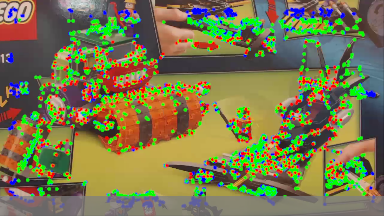
\includegraphics[height=2.5cm]{features.png} 
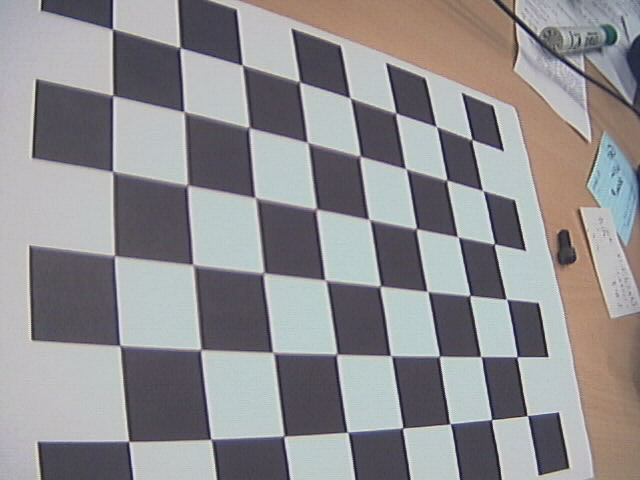
\includegraphics[height=2.5cm]{sampleOldCam.jpg}
\caption{\textbf{Left:} Features extracted using an off-the-shelf implementation. Point color denotes different scales. There is a big area around the border where no features are extracted. \textbf{Right:} Images from camera C have significant distortion.}
\label{fig:sample}
\vspace*{-0.25cm}
\end{figure}

\end{document}
